% This work is licensed under
% http://creativecommon.org/licenses/by/3.0/
\section{Examples of dynamic-routing mobility in hierarchical layers}
\label{sec:sec5}

Both of the designs in this section are intended for mobility within
the Internet core.  For this reason, both must grapple with the
problem of a hierarchical name space as explained in
Section~\ref{sec:drm}.
To reduce overhead, both solutions
significantly limit the number of routers in the Internet that must
store and update state concerning how to reach each mobile node.

\subsection{Mobile IPv4}
\label{sec:mipv4}

Mobile IPv4 \cite{mobile-IP,rfc3344} drastically reduces storage and update
costs by reducing the number of routers that must have a current route
to a particular mobile host to one or two.
Also, because each router is responsible for only a limited number of
mobile hosts, no router is over-burdened by mobility.

Figure~\ref{fig:mipv4} shows the path of a message from correspondent
host {\it C}
to mobile host {\it M} in an Internet core layer with Mobile IPv4.
Router {\it HA} is the {\it home agent} of {\it M}, and is supposed to
have a route to it at all times.
Router {\it FA} is the {\it foreign agent} of {\it M}, meaning that
it is local to the subnetwork where {\it M} is now attached,
and currently knows a route to {\it M} through the subnetwork.

\begin{figure}
\centering
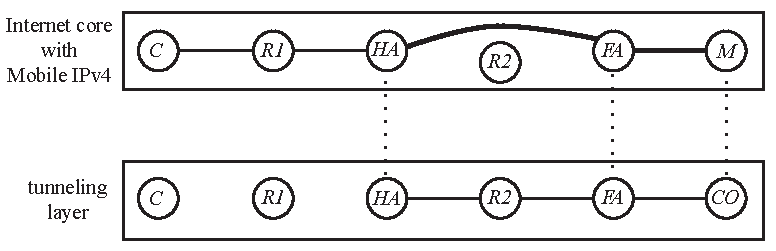
\includegraphics[scale=0.90]{figures/mipv4.pdf}
\caption{The path of a message to mobile host {\it M} with Mobile IPv4.
Special links are drawn with heavier lines.
Only the links employed in the path are shown.}
\label{fig:mipv4}
\end{figure}

The IP address {\it M} is in an aggregated routing block such that
all messages destined for the block are routed to {\it HA}.
Thus this router need only be the home agent for mobile hosts with
IP addresses in its
block.
The message from {\it C} arrives at {\it HA} by means of normal IP
routing through router {\it R1}.
The subnetwork of {\it HA} is {\it M}'s home subnetwork, so when {\it M}
is at home {\it HA} has a local route to it.

When {\it M} is not at home and becomes
attached to the subnetwork of {\it FA}, it gets a local ``care-of''
IP address {\it CO}
in that subnetwork.
{\it M} informs {\it FA},
which informs {\it HA} that it is the current foreign agent of {\it M}.
To forward messages to {\it M}, however, {\it HA} cannot merely forward
them toward {\it FA}.
It they were sent out on normal IP links, normal IP routing would send
them back to {\it HA}!
Messages to {\it M} from {\it HA} and {\it FA} must be forwarded on
special links that are separate from normal IP links.

As shown in Figure~\ref{fig:mipv4}, the special links in the Internet
core are implemented by a tunneling layer below the core layer.
The home agents, foreign agents, and mobile hosts of the Internet core
are all registered at members of the tunneling layer.
Home agents and foreign agents have the same names in both layers,
while
{\it M} is attached to member {\it CO} in the tunneling layer.
To forward a message for {\it M}
on its special link, {\it HA} in the core layer encapsulates the
message in another message destined for {\it FA}, and passes the message
to member {\it HA} in the tunneling layer.

Although the tunneling layer resembles the core layer (see below), 
its state differs from that of the core layer in several important 
respects:
\begin{itemize}
\item
{\it Routes:}
In the core layer, 
at {\it HA} messages for {\it M} are forwarded to {\it FA} on a special 
link,
at {\it FA} messages for {\it M} are forwarded to {\it M} on a special 
link,
and everywhere else messages for {\it M} are forwarded to {\it HA} on 
a normal link.
In the tunneling layer {\it M} does not exist.
\item
{\it Attachments:}
Some
members of the core layer are attached to members of the tunneling layer.
\item
{\it Locations:}
The core layer has no {\it locations} state, at least not related to
Mobile IPv4.
Although the tunneling layer need not maintain explicit
{\it locations} state for
mobile routers because they have the same names in both layers,
it must maintain explicit {\it locations} state for mobile hosts from the
core layer.
This state, which supplies the current local IP address of a mobile host,
is stored in the foreign agent to which it is relevant.
\end{itemize}

In Mobile IPv4, mobile hosts such as {\it M} send messages to their
correspondents such as {\it C} though normal IP links.
This often creates problems because IP address {\it M} is not part of
the normal routing block of the subnetwork at {\it FA}.
If there is ingress filtering for security in or near this subnet,
messages with a source address of {\it M} will be thrown away.
In Section~\ref{sec:sec7} we shall see how Mobile IPv6 eliminates this
problem.

Overall this is an interesting architecture because 
the Internet core layer and the tunneling layer
are mostly identical, and share the same
implementation.
Home agents, foreign agents, and mobile hosts are all aware of the
differences between the layers and aware of their dual membership and
dual roles.
The shared implementation works because none of the other members
of the layers need to be self-aware in that way.
They always behave the same, without knowing that sometimes their
actions contribute to the core layer, while other times their actions
contribute to the tunneling layer.

By distinguishing clearly between the two layers,
we make it possible to check the correctness of the software for each.
It also becomes possible to make further distinctions if advantageous.
For instance, implementation of a
link between {\it HA} and {\it R2} can be shared by
both layers, but it might make sense to distinguish links in the two
layers for reasons of performance or accounting.

\subsection{MSM-IP}

MSM-IP \cite{multicast} is a proposal for using IP multicast
to implement mobility.
A mobile host gets an IP address {\it M}
in the distinguished multicast block.
When the mobile host
attaches to a new subnetwork using local IP address {\it L},
{\it L} joins the multicast group for {\it M}, and the previous
local address used by {\it M} resigns from the group.

With IP multicast there is a distinguished set of multicast routers,
which are globally distributed and 
are responsible for routing messages destined for a multicast
address to all members of the address's current multicast group.
These routers exchange information and forward messages to each other
through special links,
exactly as the routers participating
in Mobile IP do.
The special links are implemented by a tunneling layer, exactly as the
special links in Mobile IP are.

With MSM-IP, every subnetwork that supports either mobile hosts or
their correspondents must have a multicast router.
Messages to mobile hosts (or true multicast groups) are recognized
by their distinguished addresses and sent to their local multicast
router, where they enter the special multicast routing 
system.

\subsection{Comparative resource costs}

The costs of dynamic-routing mobility depend greatly on the number
of routers that must have a current route to each mobile host.
More routers incur more storage and update costs.
Storage and update costs are much greater for MSM-IP than for Mobile IPv4,
because an entire network of multicast routers must be updated on each
move.

Using fewer routers, on the other hand, incurs more path cost.
With MSM-IP path cost is minimal, because a message travels from the
multicast router in the sender's subnetwork, along an optimal path 
through the distributed multicast routers, to the multicast router in
the receiver's subnetwork.
With Mobile IPv4 path cost can be high, because each message to a mobile
host must pass through the home agent, regardless of where the sender
is and where the mobile host is.
This problem of path cost or ``triangular routing'' is the reason why
the designers of Mobile IPv4 decided to send messages from mobile hosts
through normal IP links.
They incur no path cost, but they do run afoul of security
filtering.\footnote{Messages from MSM-IP mobile hosts do not have
problems with security filtering because multicast IP addresses are
recognizable as belonging to a special category.}

In Section~\ref{sec:majordifferences} we said that dynamic-routing
mobility does not in principle require participation of the endpoints.
Mobile hosts in Mobile IPv4 and MSM-IP do not have this advantage.
The reason that they must have special behavior is that both designs
use special routing mechanisms, separate from normal IP
routing, to find mobile hosts.
Because the routing mechanism is special, it is not necessary to
update every IP router when a mobile host moves.
But also, because the routing mechanism is special, mobile hosts must also
behave differently to interact with it in the correct way.
